%%%%%%%%%%%%%%%%%%%%%%%%%%%%%%%%%%%%%%%%%%%%%%%%%%%%%%%%%%%%%%%%%%%%%%%%%%%%%
%%% LaTeX-Rahmen fuer das Erstellen von Masterarbeiten
%%%%%%%%%%%%%%%%%%%%%%%%%%%%%%%%%%%%%%%%%%%%%%%%%%%%%%%%%%%%%%%%%%%%%%%%%%%%%

%%%%%%%%%%%%%%%%%%%%%%%%%%%%%%%%%%%%%%%%%%%%%%%%%%%%%%%%%%%%%%%%%%%%%%%%%%%%%
%%% allgemeine Einstellungen
%%%%%%%%%%%%%%%%%%%%%%%%%%%%%%%%%%%%%%%%%%%%%%%%%%%%%%%%%%%%%%%%%%%%%%%%%%%%%

\documentclass[twoside,12pt,a4paper]{report}
%\usepackage{reportpage}
\usepackage{amsmath}
\usepackage{amssymb}
\usepackage{stmaryrd}
\usepackage{mathrsfs}
\usepackage{scalerel}
\usepackage{epsf}
\usepackage{graphics, graphicx}
\usepackage{latexsym}
\usepackage[margin=10pt,font=small,labelfont=bf]{caption}
\usepackage[utf8]{inputenc}
\usepackage[toc,page]{appendix}
\usepackage{subcaption}
\usepackage{tikz-cd}
\usetikzlibrary{cd}

\usepackage{amsthm}
\newtheorem{definition}{Definition}

\usepackage[hyphens]{url} % 'hyphens' option allows line breaks after "-" characters
\usepackage[ colorlinks = true
           , linkcolor = black
           , anchorcolor = black
           , citecolor = black
           , urlcolor = blue]{hyperref}

\usepackage{lineno}
\linenumbers
\usepackage{listings}
% basic duo style
\lstdefinestyle{duoStyle}{%
    morekeywords={if, then, else instance, class, >>, CBV, CBN, +, -, =>, case, of, cocase, mu, def, prd, cns, cmd, :=},
    keywordstyle=\ttfamily\bfseries\color{blue!80!black},
    mathescape=true
    %moredelim=**[is][\bfseries]{|}{|}
}
\lstset{style=duoStyle}

\usepackage{minted}


\usepackage{bussproofs}
\EnableBpAbbreviations
\def\ScoreOverhang{0pt}
\def\buildNoScoreTight{% Make an hbox with no score
 \global\setbox\myBoxD=\hbox{\vbox{\vskip0pt}}% 0pt instead of 1pt
}
\def\noLine{% noLine with less space between lines
 \gdef\buildScore{\buildNoScoreTight}%
 \ignorespaces%
}

% Inference rules
\newcommand{\subPosRule}{\RightLabel{\textsc{Sub}$^+$}}
\newcommand{\subNegRule}{\RightLabel{\textsc{Sub}$^-$}}
\newcommand{\instanceDeclRule}{\RightLabel{\textsc{Decl}}}
\newcommand{\meetRule}{\RightLabel{\textsc{Meet}}}
\newcommand{\joinRule}{\RightLabel{\textsc{Join}}}
\newcommand{\axiomPos}{\RightLabel{\textsc{Axiom}$^+$}}
\newcommand{\axiomNeg}{\RightLabel{\textsc{Axiom}$^-$}}
\newcommand{\topRule}{\RightLabel{\textsc{Top}}}
\newcommand{\botRule}{\RightLabel{\textsc{Bot}}}

\newcommand\deriveRule{
  {\hskip.1in}
  $\stackrel{\mathit{drv}}{\rightsquigarrow}$
  {\hskip.1in}}

\newcommand{\ctx}{\ensuremath{\Gamma \; \vdash \;}}
\newcommand{\opeq}{\ensuremath{\stackrel{op}{\simeq}}}

% Symbols
\newcommand\join{\vee}
\newcommand\meet{\wedge}
\newcommand\sub{\ensuremath{\leqslant}}

% Text
\newcommand\Showable{\ensuremath{\Psi_\mathit{Show}}}
\newcommand\Defaultable{\ensuremath{\Psi_\mathit{Default}}}
\newcommand\instance[2]{{\bf instance} \; #1(#2)}

% Terms
\newcommand\caseof[1]{{\bf case}\; #1 \;{\bf of}}
\newcommand\showTerm{{\bf show}\;}
\newcommand\eq{{\bf eq}\;}

% Types
\newcommand\Nat{\mathbb{N}}
\newcommand\Int{\mathbb{Z}}
\newcommand\Unit{\mathbb{U}}
\newcommand\Bool{\mathbb{B}}
\newcommand\String{\mathit{String}}

% Witnesses
\newcommand\cov{\mathit{cov}}
\newcommand\contrav{\mathit{contrav}}
% relational composition operator
\newcommand*{\comp}{\mathbin{\raise 0.6ex\hbox{\oalign{\hfil$\scriptscriptstyle
            		 \rm o$\hfil\cr\hfil$\scriptscriptstyle\rm 9$\hfil}}}}
\newcommand\refl{\mathit{refl}}
\newcommand\topW{\mathit{top}}
\newcommand\natPrim{\mathit{natPrim}}
\newcommand\botW{\mathit{bot}}
\newcommand\meetW{\mathit{meet}}
\newcommand\joinW{\mathit{join}}
\newcommand\inW[1]{\mathit{in}_{#1}}
\newcommand\proj[1]{\mathit{proj}_{#1}}
\newcommand\funcW{\mathit{func}}
\newcommand\unfoldL{\mathit{unfold}_{L}}
\newcommand\unfoldR{\mathit{unfold}_{R}}

\newcommand\constraintGen[1]{\ensuremath{\llbracket #1 \rrbracket}}
\newcommand\toConstr{\ensuremath{\hookrightarrow}}
\newcommand\decompose[2]{\ensuremath{{\mathbf{decompose}}(#1 \sub #2)}}

\usepackage{mathpartir}

\textwidth 14cm
\textheight 22cm
\topmargin 0.0cm
\evensidemargin 1cm
\oddsidemargin 1cm
%\footskip 2cm
\parskip0.5explus0.1exminus0.1ex

% Kann von Student auch nach pers\"onlichem Geschmack ver\"andert werden.
\pagestyle{headings}

\sloppy

% not working as intended
% \newcommand{\textHaskell}{1}{\mint{Haskell}|$1|}

\begin{document}

%%%%%%%%%%%%%%%%%%%%%%%%%%%%%%%%%%%%%%%%%%%%%%%%%%%%%%%%%%%%%%%%%%%%%%%%%%%%
%%% hier steht die neue Titelseite 
%%%%%%%%%%%%%%%%%%%%%%%%%%%%%%%%%%%%%%%%%%%%%%%%%%%%%%%%%%%%%%%%%%%%%%%%%%%%
 
\begin{titlepage}
 \begin{center}
  {\LARGE Eberhard Karls Universit\"at T\"ubingen}\\
  {\large Mathematisch-Naturwissenschaftliche Fakult\"at \\
Wilhelm-Schickard-Institut f\"ur Informatik\\[4cm]}
  {\huge Master Thesis Informatics\\[2cm]}
  {\Large\bf  Type Class Coherence with Subtyping\\[1.5cm]}
 {\large Pascal Engel}\\[0.5cm]
Datum\\[4cm]
{\small\bf Reviewers}\\[0.5cm]
  \parbox{7cm}{\begin{center}{\large Name Erstgutachter}\\
   (Informatik)\\
  {\footnotesize Wilhelm-Schickard-Institut f\"ur Informatik\\
	Universit\"at T\"ubingen}\end{center}}\hfill\parbox{7cm}{\begin{center}
  {\large Name Zweitgutachter}\\
  (Informatik)\\
  {\footnotesize Wilhelm-Schickard-Institut f\"ur Informatik\\
	Universit\"at T\"ubingen}\end{center}
 }
  \end{center}
\end{titlepage}

%%%%%%%%%%%%%%%%%%%%%%%%%%%%%%%%%%%%%%%%%%%%%%%%%%%%%%%%%%%%%%%%%%%%%%%%%%%%
%%% Titelr"uckseite: Bibliographische Angaben
%%%%%%%%%%%%%%%%%%%%%%%%%%%%%%%%%%%%%%%%%%%%%%%%%%%%%%%%%%%%%%%%%%%%%%%%%%%%

\thispagestyle{empty}
\vspace*{\fill}
\begin{minipage}{11.2cm}
\textbf{Engel, Pascal:}\\
\emph{Type Class Coherence with Subtyping}\\ Master Thesis Informatics\\
Eberhard Karls Universit\"at T\"ubingen\\
Thesis period: von-bis
\end{minipage}
\newpage

%%%%%%%%%%%%%%%%%%%%%%%%%%%%%%%%%%%%%%%%%%%%%%%%%%%%%%%%%%%%%%%%%%%%%%%%%%%%

\pagenumbering{roman}
\setcounter{page}{1}

%%%%%%%%%%%%%%%%%%%%%%%%%%%%%%%%%%%%%%%%%%%%%%%%%%%%%%%%%%%%%%%%%%%%%%%%%%%%
%%% Seite I: Zusammenfassug, Danksagung
%%%%%%%%%%%%%%%%%%%%%%%%%%%%%%%%%%%%%%%%%%%%%%%%%%%%%%%%%%%%%%%%%%%%%%%%%%%%


\section*{Abstract}

In this work we aim to bring together three notions of polymorphism:
Subtyping as a form of ad hoc polymorphism, parametric polymorphism and type classes.
We do so by extending the research language \texttt{duo}, which already supports algebraic subtyping, with type classes.
In order to ensure type class coherence we argue for a restrictive way of implementing instances for types that are in the subtyping relation.

% \newpage
% \section*{Acknowledgements}

% Write here your acknowledgements.

\cleardoublepage

%%%%%%%%%%%%%%%%%%%%%%%%%%%%%%%%%%%%%%%%%%%%%%%%%%%%%%%%%%%%%%%%%%%%%%%%%%%%%
%%% Table of Contents
%%%%%%%%%%%%%%%%%%%%%%%%%%%%%%%%%%%%%%%%%%%%%%%%%%%%%%%%%%%%%%%%%%%%%%%%%%%%%

\renewcommand{\baselinestretch}{1.3}
\small\normalsize

\tableofcontents

\renewcommand{\baselinestretch}{1}
\small\normalsize

\cleardoublepage

%%%%%%%%%%%%%%%%%%%%%%%%%%%%%%%%%%%%%%%%%%%%%%%%%%%%%%%%%%%%%%%%%%%%%%%%%%%%%
%%% Der Haupttext, ab hier mit arabischer Numerierung
%%% Mit \input{dateiname} werden die Datei `dateiname' eingebunden
%%%%%%%%%%%%%%%%%%%%%%%%%%%%%%%%%%%%%%%%%%%%%%%%%%%%%%%%%%%%%%%%%%%%%%%%%%%%%

\pagenumbering{arabic}
\setcounter{page}{1}

%% Introduction
%%%%%%%%%%%%%%%%%%%%%%%%%%%%%%%%%%%%%%%%%%%%%%%%%%%%%%%%%%%%%%%%%%%%
% Introduction
%%%%%%%%%%%%%%%%%%%%%%%%%%%%%%%%%%%%%%%%%%%%%%%%%%%%%%%%%%%%%%%%%%%%

\chapter{Introduction}\label{ch:intro}

% this section likely needs a big overhaul
In many functional programming languages such as Haskell, type classes are a powerful tool to generalize functions over different data types.
This allows us e.g. to use the \mintinline{Haskell}|+| operator both on \mintinline{Haskell}|Int| and \mintinline{Haskell}|Float| types.
Another approach to overloading functions is subtyping, i.e. if a value of a certain type is expected we can also supply a value of a more specific type that is subsumed by the general type.
For example, since the type of natural numbers \mintinline{text}|Nat| is a subtype of the integers \mintinline{text}|Int|, we can supply a value of type \mintinline{text}|Nat| for any function that expects an \mintinline{text}|Int|.

Although these approaches do not serve exactly the same purpose it is uncommon to find both concepts in the same language.
In this work, I am going to show how it is possible to implement type classes in a language that supports subtyping.
There are unique challenges when bringing both together because instances for certain types are going to be ambiguous.

The Haskell type \mintinline{Haskell}|Either a b| roughly corresponds to the lattice type \mintinline{text}|a \/ b|.
Given a type class \mintinline{Haskell}|C :: * -> *| and instances \mintinline{Haskell}|C a| and \mintinline{Haskell}|C b| the instance \mintinline{Haskell}|C (Either a b)| has to be defined by hand which can be easily done by pattern-matching and using the given instances.
However, instances for lattice types are neither explicit nor straightforward:
Since \mintinline{text}|a \/ b| does not have a uniquely-determined(?) constructor we might just implicitly derive \mintinline{text}|C (a \/ b)| from the given instances.
However, this would make instances undecidable if we later on decide to implement an explicit instance of \mintinline{text}|C (a \/ b)|.

Together with subtyping we may be able to overload type classes even more.
Consider
\begin{minted}{text}
    Show(if b then 42 : Nat else "Hello World" : String)
\end{minted}
This term of type \mintinline{text}{Nat \/ String} appears to be well typed iff we can resolve the type class instances for \mintinline{text}{Show Nat} and \mintinline{text}{Show String}.

In the following we will explore how type classes interact with these and other lattice types.

\cleardoublepage

%%
\chapter{Polymorphism}\label{ch:polymorphism}

In order to generalize functions over data types there have been several proposals to abstract over types in different programming languages:
These can be summarised in three categories: parametric polymorphism, subtyping and ad-hoc polymorphism.

\section{Parametric polymorphism}\label{sec:parmetric-polymorphism}

We can define functions without knowing the concrete representation of the arguments and result types (e.g. \texttt{id : a -> a}) % cite something
Abstract algorithms detached from concrete type representation.
Allows for 'theorems for free'. \cite{wadlertheorems}

\section{Subtyping}\label{sec:subtyping}

In many cases the specific semantics of types exhibit a hierarchy.
In Object-oriented programming this hierarchy is given in the form of sub- and superclasses.
We can express the relationship between super- and subclasses, or more generally super- and subtypes,
in the form that all properties of the superclass is also exhibited in the subclass. \cite{subtyping}

In the case of OO-languages this means that, if the class \texttt{SubC} is a subclass of \texttt{SuperC},
then any method defined in \texttt{SuperC} is also going to be defined for objects of \texttt{SubC}.
This enables us to use an object \texttt{SubC} wherever a \texttt{SuperC} is expected.

We denote $T \leq S$ for $T$ is a subtype of $S$.
Syntactically, this implies that if we have obatined the judgement $e : T$, we also have $e : S$.
Therefore, we can use $e$ in any context that expects the usage of a term of type $S$.
Semantically, the subtyping relation can be understood analogously to sets in terms of the subset relationship $\subseteq$,
meaning all terms $e$ of type $T$ are also of type $S$.
\cite{reynolds_1998}

This permits many useful features in programming languages such as the reuse and abstraction of code to the supertypes and implicit coercions from a subtype to a supertype.


\section{Ad-hoc polymorphism}\label{sec:ad-hoc-polymorphism}
% overloading vs type classes
% paper by wadler

In some - mostly imperative - languages it is possible to simply overload functions (e.g. we may define \texttt{+} both on integers and on float values, the correct implementation is then picked based on the argument type).
However, there is usually no way to express this in the type system of these languages. % cite...

If our type system doesn't allow for ad-hoc polymorphism it may seem neccessary to write verbose code for basic function with respect to every concrete type it should be used for.
An intuitive example for this (that is also the motivation for type classes in the original proposal) are arithmetic operators.
We simply cannot define \texttt{(+) : Int -> Int -> Int} and then also \texttt{(+) : Float -> Float -> Float} in a different implementation, on which both types definetly rely on under the hood.
But these types have nonetheless something in common. Namely that they both stand for \emph{numerical} values, that hence support the usual arithmetic operations, like addition, multiplication, division and so on.

The idea of type classes is to generalise attributes of types with appropriate function.
The class \mintinline{Haskell}|Num| in Haskell expects that we can implement a number of numerical functions for a type $\tau$ if it is ought to be a member of the \mintinline{Haskell}|Num| type class.

Shortened definition of the \mintinline{Haskell}|Num| type class in Haskell.
\footnote{As can be found in the default \texttt{Prelude}: \url{https://hackage.haskell.org/package/base-4.16.2.0/docs/Prelude.html\#t:Num}}

\begin{minted}{Haskell}
class  Num a  where
    (+), (-), (*) :: a -> a -> a
\end{minted}

An instance would look like:

\begin{minted}{Haskell}
instance  Num Int  where
    (+) = intAdd
    (-) = intMinus
    (*) = intMul
\end{minted}





% later:
% category theory: functors, monoids, monads, etc.

In the end, this enables us to use elaborate concepts such as functors and monads to reason about programs.

\cite{wadlerblott}

\section{The problem of type class coherence}\label{sec:coherence}
% for each type there t may be globally at most one instance C t defined
% discuss overlapping instances
% can already be tricky in a modular system
% more challenging with subtyping

Even though the general concept of type classes introduces a general meaning for each type class.
The evaluation still strongly depends on implementation details found in specific instances.
For example, for the \texttt{Ord} type class we may choose to implement the ordering in ascending or descending order.
It is therefore crucial, that for each type the corresponding instance - if it exists - is uniquely determined by the type.

Reynolds \cite{reynolds_coherence} describes the issue of coherence as follows:

\begin{quote}
    When a programming language has a sufficiently rich type structure, there can be more than one proof of the same
    typing judgment; potentially this can lead to semantic ambiguity since the semantics of a typed language is a function
    of such proofs. When no such ambiguity arises, we say that the language is coherent.
\end{quote}

For type classes, this means that no two instances should be able to be resolved for the same type.
A rather obvious example would be to define two different instances for the same type.
For example one instance of \mintinline{Haskell}{Ord Int}, one with ascending and one with descending order.
The ambiguity arises as soon as we make use of these instances and it is no longer clear which one should be picked for evaluation.

More surprisingly type class coherence is already violated for overlapping instances.
As part of the standard prelude we find both \mintinline{Haskell}{instance Show a => Show [a]} and \mintinline{Haskell}{instance Show String}
(with \mintinline{Haskell}{String} being a type synonym for \mintinline{Haskell}{[Char]}).
The \texttt{Show} instance for Strings differs from the more general instance for lists.

Ambiguous programs should generally not be typeable.
One example, also mentioned in the Haskell 98 report \cite{Haskell98} is this short program which simply reads a string to a data type and then converts it back to string without specifying which data type is being used:

\begin{minted}{Haskell}
    f :: String -> String
    f str = let x = read str in show x
\end{minted}

There may be multiple types that satisfy the type class constraints.
The specific implementation of \mintinline{Haskell}{show :: forall a. (Show a) => a -> String} and \mintinline{Haskell}{read :: forall a.(Read a) -> String -> a} is therefore unknown.

In the Haskell98 standard, type class coherence is guaranteed by the syntactical equivalence of resolved instances.
For each Haskell type there may be at most one instance defined for each type class.


\subsection{Example}

Consider superclasses in Haskell.
E.g. the type class \mintinline{Haskell}{Eq} is a superclass of \mintinline{Haskell}{Ord}, written \mintinline{Haskell}{Eq a => Ord a}.
This means that for each type that we want to define an ordering for already needs to have equality defined on.

For example, given an instance for \mintinline{Haskell}{Ord (Maybe a)} we can then derive that an instance for \mintinline{Haskell}{Eq a} has to exist.
As shown in the diagram, we can take different paths to do so but type class coherence guarantees that no matter which path we choose to resolve the instance, we will always find \emph{the same} instance.
In Haskell98 type class coherence guarantees that all such diagrams commute.
So even if there may be different ways to resolve type class constraints, all of them preserve the same semantics.

\begin{tikzcd}
    &  & \mintinline{Haskell}|Ord (Maybe a)| \arrow[llddd, "{\footnotesize\mintinline{Haskell}|class Eq a => Ord a|}"'] \arrow[rrddd, "{\footnotesize\mintinline{Haskell}|instance Ord a => Ord (Maybe a)|}"] &  &                            \\
    &  &                                &  &                            \\
    &  &                                &  &                            \\
    \mintinline{Haskell}|Eq (Maybe a)| \arrow[rrddd, "{\footnotesize\mintinline{Haskell}|instance Eq a => Eq (Maybe a)|}"'] &  &                                &  & \mintinline{Haskell}|Ord a| \arrow[llddd, "{\footnotesize \mintinline{Haskell}|class Eq a => Ord a|}"] \\
    &  &                                &  &                            \\
    &  &                                &  &                            \\
    &  & \mintinline{Haskell}|Eq a|                  &  &                           
\end{tikzcd}

Even though there are multiple ways to derive an instance for \mintinline{Haskell}|Eq a| from an instance of \texttt{Ord (Maybe a)}, the derived instance has to be uniquely determined.
Since the diagram commutes, there has to be exactly one instance for \mintinline{Haskell}|Eq a|.

Uniqueness or non-ambiguity of type classes.

\cleardoublepage

%% 
\chapter{Qualified Types}
\label{ch:qualified-types}

\section{Theory of Predicates}

To reason about ad-hoc polymorhism we talk about \emph{qualified types}, i.e. types that satisfy some predicate.

\begin{definition} Predicates\\
  Given a universe of types $\Unit$, a \emph{predicate over types} $\Phi$ is an element of $\mathcal{P}(\Unit)$.
\end{definition}

We are only interested in predicates that are preserved over the subtyping lattice.
I.e. predicates that depend only on the terms of a type.
That means only predicates that are \emph{monotonous} are considered while other predicates such as \emph{"has exactly two values"} are disregarded.
We further differentiate between \emph{covariant} and \emph{contravariant} predicates over types.

Let $\Gamma$ be the context of facts, i.e. known types that satisfy specific predicates.

\begin{definition}
  A \emph{covariant type class predicate} $\Phi^+$ is a predicate preserved by the subtyping relation, i.e. it adheres to the following rule:
\end{definition}

% The monotonicity of $\Phi^+$ motivates the following rule preserving the predicate for subtypes.
% From the definition of covariant predicates it follows that $\phi$ holds for every term of $\sigma$ and because every witness of $\tau$ is also a witness of $\sigma$ the characteristic property $\phi$ holds for all witnesses of $\tau$.

% ^< statt ^+

\begin{prooftree}
  \AxiomC{$\ctx \Phi^+(\sigma)$}
  \AxiomC{$\tau \sub \sigma$}
  \alwaysSingleLine
  \RightLabel{\textsc{CoV}}
  \BinaryInfC{$\ctx \Phi^+(\tau)$}
\end{prooftree}

With \textsc{CoV} and the subtyping rules in fig. \ref{fig:subtyping} we can derive several useful rules:

\begin{figure}[h]
\begin{center}
  \AxiomC{$\ctx \Phi^+(\top)$}
  \AxiomC{}
  \RightLabel{\textsc{Top}}
  \UnaryInfC{$\tau \sub \top$}
  \alwaysSingleLine
  \RightLabel{\textsc{CoV}}
  \BinaryInfC{$\ctx \Phi^+(\tau)$}
  \DisplayProof
  \deriveRule
  \AxiomC{$\ctx \Phi^+(\top)$}
  \alwaysSingleLine
  \RightLabel{\textsc{Top}$^+$}
  \UnaryInfC{$\ctx \Phi^+(\tau)$}
  \DisplayProof
\end{center}

\begin{center}
  \AxiomC{$\ctx \Phi^+(\tau)$}
  \AxiomC{}
  \RightLabel{\textsc{Bot}}
  \UnaryInfC{$\bot \sub \tau$}
  \alwaysSingleLine
  \RightLabel{\textsc{CoV}}
  \BinaryInfC{$\ctx \Phi^+(\bot)$}
  \DisplayProof
  \deriveRule
  \AxiomC{$\ctx \Phi^+(\tau)$}
  \alwaysSingleLine
  \RightLabel{\textsc{Bot}$^+$}
  \UnaryInfC{$\ctx \Phi^+(\bot)$}
  \DisplayProof
\end{center}

\begin{center}
  \AxiomC{$\ctx \Phi^+(\tau)$}
  \AxiomC{}
  \RightLabel{\textsc{Refl}}
  \UnaryInfC{$\tau \sub \tau$}
  \RightLabel{\textsc{MeetI}$_1$}
  \UnaryInfC{$\tau \meet \sigma \sub \tau$}
  \alwaysSingleLine
  \RightLabel{\textsc{CoV}}
  \BinaryInfC{$\ctx \Phi^+(\tau \meet \sigma)$}
  \DisplayProof
  \deriveRule
  \AxiomC{$\ctx \Phi^+(\tau)$}
  \alwaysSingleLine
  \RightLabel{\textsc{Meet}$_1^+$}
  \UnaryInfC{$\ctx \Phi^+(\tau \meet \sigma)$}
  \DisplayProof
\end{center}

\begin{center}
  \AxiomC{$\ctx \Phi^+(\tau)$}
  \AxiomC{}
  \RightLabel{\textsc{Refl}}
  \UnaryInfC{$\tau \sub \tau$}
  \RightLabel{\textsc{MeetI}$_2$}
  \UnaryInfC{$\sigma \meet \tau \sub \tau$}
  \alwaysSingleLine
  \RightLabel{\textsc{CoV}}
  \BinaryInfC{$\ctx \Phi^+(\sigma \meet \tau)$}
  \DisplayProof
  \deriveRule
  \AxiomC{$\ctx \Phi^+(\tau)$}
  \alwaysSingleLine
  \RightLabel{\textsc{Meet}$_2^+$}
  \UnaryInfC{$\ctx \Phi^+(\sigma \meet \tau)$}
  \DisplayProof
\end{center}

\begin{center}
  \AxiomC{$\ctx \Phi^+(\Int)$}
  \AxiomC{}
  \RightLabel{\textsc{NatPrim}}
  \UnaryInfC{$\Nat \sub \Int$}
  \alwaysSingleLine
  \RightLabel{\textsc{CoV}}
  \BinaryInfC{$\ctx \Phi^+(\Nat)$}
  \DisplayProof
  \deriveRule
  \AxiomC{$\ctx \Phi^+(\Int)$}
  \alwaysSingleLine
  \RightLabel{\textsc{NatPrim}$^+$}
  \UnaryInfC{$\ctx \Phi^+(\Nat)$}
  \DisplayProof
\end{center}

\label{fig:derived-covariant-rules}
\caption{Derived rules for covariant predicates}
\end{figure}

A typical example for covariant predicates is $\Showable$: all types that are showable, which generally rules out function types.
The \textsc{CoV} rule seems intuitive for this:
If $e : \tau$ is a showable term and $\tau \sub \sigma$, then $e : \sigma$ can be shown in the same way.

\begin{definition}
  A \emph{contravariant type class predicate} $\Phi^-$ is a predicate preserved by the supertyping or flipped subtyping relation, i.e. it adheres to the following rule:
\end{definition}

\begin{prooftree}
  \alwaysNoLine
  \AxiomC{$\ctx \Phi^-(\sigma)$}
  \AxiomC{$\sigma \sub \tau$}
  \alwaysSingleLine
  \RightLabel{\textsc{ContraV}}
  \BinaryInfC{$\ctx \Phi^-(\tau)$}
\end{prooftree}

The rules for contravariant predicates are dual to those for covariant predicates.
The monotonicity of $\Phi^-$ motivates the following rule preserving the predicate for supertypes:
From the definition of contravariant predicates it follows that $\phi$ holds for some term of $\sigma$ and because every witness of $\sigma$ is also a witness of $\tau$ there is at least one witness of $\tau$ for which the characteristic property $\phi$ holds.

With \textsc{ContraV} and the subtyping rules in fig. \ref{fig:subtyping} we can again derive several useful rules:

\begin{figure}[h]
\begin{center}
  \AxiomC{$\ctx \Phi^-(\tau)$}
  \AxiomC{}
  \RightLabel{\textsc{Top}}
  \UnaryInfC{$\tau \sub \top$}
  \alwaysSingleLine
  \RightLabel{\textsc{ContraV}}
  \BinaryInfC{$\ctx \Phi^-(\top)$}
  \DisplayProof
  \deriveRule
  \AxiomC{$\ctx \Phi^-(\tau)$}
  \alwaysSingleLine
  \RightLabel{\textsc{Top}$^-$}
  \UnaryInfC{$\ctx \Phi^-(\top)$}
  \DisplayProof
\end{center}

\begin{center}
  \AxiomC{$\ctx \Phi^-(\bot)$}
  \AxiomC{}
  \RightLabel{\textsc{Bot}}
  \UnaryInfC{$\bot \sub \tau$}
  \alwaysSingleLine
  \RightLabel{\textsc{ContraV}}
  \BinaryInfC{$\ctx \Phi^-(\tau)$}
  \DisplayProof
  \deriveRule
  \AxiomC{$\ctx \Phi^-(\bot)$}
  \alwaysSingleLine
  \RightLabel{\textsc{Bot}$^-$}
  \UnaryInfC{$\ctx \Phi^-(\tau)$}
  \DisplayProof
\end{center}

\begin{center}
  \AxiomC{$\ctx \Phi^-(\tau)$}
  \AxiomC{}
  \RightLabel{\textsc{Refl}}
  \UnaryInfC{$\tau \sub \tau$}
  \RightLabel{\textsc{JoinI}$_1$}
  \UnaryInfC{$\tau \sub \tau \join \sigma$}
  \alwaysSingleLine
  \RightLabel{\textsc{ContraV}}
  \BinaryInfC{$\ctx \Phi^-(\tau \join \sigma)$}
  \DisplayProof
  \deriveRule
  \AxiomC{$\ctx \Phi^-(\tau)$}
  \alwaysSingleLine
  \RightLabel{\textsc{Join}$_1^-$}
  \UnaryInfC{$\ctx \Phi^-(\tau \join \sigma)$}
  \DisplayProof
\end{center}

\begin{center}
  \AxiomC{$\ctx \Phi^-(\tau)$}
  \AxiomC{}
  \RightLabel{\textsc{Refl}}
  \UnaryInfC{$\tau \sub \tau$}
  \RightLabel{\textsc{JoinI}$_2$}
  \UnaryInfC{$\tau \sub \sigma \join \tau$}
  \alwaysSingleLine
  \RightLabel{\textsc{ContraV}}
  \BinaryInfC{$\ctx \Phi^-(\sigma \join \tau)$}
  \DisplayProof
  \deriveRule
  \AxiomC{$\ctx \Phi^-(\tau)$}
  \alwaysSingleLine
  \RightLabel{\textsc{Join}$_2^-$}
  \UnaryInfC{$\ctx \Phi^-(\sigma \join \tau)$}
  \DisplayProof
\end{center}

\begin{center}
  \AxiomC{$\ctx \Phi^-(\Nat)$}
  \AxiomC{}
  \RightLabel{\textsc{NatPrim}}
  \UnaryInfC{$\Nat \sub \Int$}
  \alwaysSingleLine
  \RightLabel{\textsc{ContraV}}
  \BinaryInfC{$\ctx \Phi^-(\Int)$}
  \DisplayProof
  \deriveRule
  \AxiomC{$\ctx \Phi^-(\Nat)$}
  \alwaysSingleLine
  \RightLabel{\textsc{NatPrim}$^-$}
  \UnaryInfC{$\ctx \Phi^-(\Int)$}
  \DisplayProof
\end{center}
\label{fig:contravariant-derived-rules}
\caption{Derived rules for contravariant predicates}
\end{figure}

A typical example for covariant predicates is $\Defaultable$: all types for which some default value can be predefined, which also generally rules out function types and empty types.
The \textsc{ContraV} again rule seems intuitive for this:
% fix:
If $e : \tau$ is a default value for $\tau$ and $\sigma \sub \tau$, then $e : \sigma$ can be used as a default value for $\sigma$ as well.


% \begin{center}
%   \alwaysNoLine
%   \AxiomC{$\ctx \Phi^-(\tau \meet \sigma)$}
%   \alwaysSingleLine
%   \RightLabel{\textsc{Meet}$_1^-$}
%   \UnaryInfC{$\ctx \Phi^-(\tau)$}
%   \DisplayProof
%   {\hskip.2in}
%   \alwaysNoLine
%   \AxiomC{$\ctx \Phi^-(\tau \meet \sigma)$}
%   \alwaysSingleLine
%   \RightLabel{\textsc{Meet}$_2^-$}
%   \UnaryInfC{$\ctx \Phi^-(\sigma)$}
%   \DisplayProof
% \end{center}

We omit the $^+$ and $^-$ superscripts if the variance of predicates does not matter.
Using this notation we can simplify axioms and the rule for constraints.
The rule for axioms is trivial: We can resolve known facts directly from the context.

  \begin{prooftree}
    \AxiomC{}
    \RightLabel{\textsc{Axiom}}
    \UnaryInfC{$\Gamma, \Phi(\tau) \vdash \Phi(\tau)$}
  \end{prooftree}

\begin{definition}
  An \emph{invariant type class predicate} $\Phi^-$ is a predicate preserved by the subtyping \emph{and} flipped subtyping relation, i.e. it adheres to the following rule:
\end{definition}
  
\begin{prooftree}
  \alwaysNoLine
  \AxiomC{$\ctx \Phi(\sigma)$}
  \AxiomC{$\sigma \sub \tau$}
  \AxiomC{$\tau \sub \sigma$}
  \alwaysSingleLine
  \RightLabel{\textsc{InV}}
  \TrinaryInfC{$\ctx \Phi(\tau)$}
\end{prooftree}

Invariant type class predicates can essentially only be derived from type equalitites, i.e. where a type is both a sub- and supertype of another.
Hence, there are no interesting derivable rules for them.

Predicates may be constrained, i.e. they depend on other predicates.
$\Phi(\tau) \Rightarrow \Psi(\tau)$ means $\Psi$ is constrained by $\Phi$.
Thus, if $\Psi(\tau)$ is satisfied, then the constraint $\Phi(\tau)$ is satisfied as well.
Note that this corresponds to implications even though the arrow is flipped as it is oriented towards constraints.

  \begin{prooftree}
    \AxiomC{$\ctx \Psi(\tau)$}
    \AxiomC{$\ctx \Phi(\tau) \Rightarrow \Psi(\tau)$}
    \RightLabel{\textsc{Constr}}
    \BinaryInfC{$\Gamma \vdash \Phi(\tau)$}
  \end{prooftree}

\subsection{Examples}

Consider the predicates $\Showable$ and $\Defaultable$.
A type $\tau$ satsifies the covariant predicate $\Showable$ if a total function of $\tau \to String$ can be defined.
Dually, a type $\tau$ satsifies the contravariant predicate $\Defaultable$ if a function of type $Unit \to \tau$ can be defined.

Let context $\Gamma := \{ \Showable(\Int), \Defaultable(\Nat) \}$.
We obtain the following derivations for $\Showable(\Singleton{1} \meet \Nat)$ and $\Defaultable(\Int \join \Bool)$:
We can interpret these derivations as a proof for \emph{Given a way to show an integer, we can also show anything that is both a natural number and of the singleton type $\Singleton{1}$} and
\emph{Given a default value for $\Nat$, we also obtain a default value for the union of $\Int$ and $\Bool$}

\begin{figure}[h]
\begin{prooftree}
  \AxiomC{}
  \RightLabel{\textsc{Axiom}}
  \UnaryInfC{$\ctx \Showable(\Int)$}
  \RightLabel{\textsc{Prim}$^+$}
  \UnaryInfC{$\ctx \Showable(\Nat)$}
  \RightLabel{\textsc{Meet}$^+_2$}
  \UnaryInfC{$\ctx \Showable(\Singleton{1} \meet \Nat)$}
\end{prooftree}
\label{fig:example-showable}
\caption{Derivation for $\ctx \Showable(\Unit \meet \Nat)$}
\end{figure}

\begin{figure}[h]
\begin{prooftree}
  \AxiomC{}
  \RightLabel{\textsc{Axiom}}
  \UnaryInfC{$\ctx \Defaultable(\Nat)$}
  \RightLabel{\textsc{Prim}$^-$}
  \UnaryInfC{$\ctx \Defaultable(\Int)$}
  \alwaysSingleLine
  \RightLabel{\textsc{Join}$^-_1$}
  \UnaryInfC{$\ctx \Defaultable(\Int \join \Bool)$}
\end{prooftree}
\label{fig:example-defaultable}
\caption{Derivation for $\ctx \Defaultable(\Int \join \Bool)$}
\end{figure}
\section{Witnesses}
\label{sec:witnesses}

By annotating applications of predicates with specific witnesses we obtain a calculus
that is not only able to prove that a type satisfies a predicate but also constructs a witness for such a proof.

This directly corresponds to type class resolution if we interpret type classes as predicates on types.
We again differentiate co- and contravariant type classes in order to transport type classes over the subtyping relation.

\begin{figure}[h]
  % refl
  \begin{prooftree}
    \AxiomC{}
    \RightLabel{\textsc{Refl}}
    \UnaryInfC{$\refl_\tau : \tau \sub \tau$}
  \end{prooftree}

  % trans
  \begin{prooftree}
    \AxiomC{$f : \tau \sub \sigma$}
    \AxiomC{$g : \sigma \sub \rho$}
    \RightLabel{\textsc{Trans}}
    \BinaryInfC{$f \comp g : \tau \sub \rho$}
  \end{prooftree}

  % top/bot
 \begin{center}
  \AxiomC{}
  \RightLabel{\textsc{Top}}
  \UnaryInfC{$\topW_\tau : \tau \sub \top$}
  \DisplayProof
  {\hskip.2in}
  \AxiomC{}
  \RightLabel{\textsc{Bot}}
  \UnaryInfC{$\botW_\tau : \bot \sub \tau$}
  \DisplayProof
\end{center}

 % join intro
 \begin{center}
    \AxiomC{$f : \tau \sub \sigma$}
    \RightLabel{\textsc{JoinI}$_1$}
    \UnaryInfC{$\inW{1}(f) : \tau \sub \sigma \join \rho$}
    \DisplayProof
    {\hskip.2in}
    \AxiomC{$f: \tau \sub \sigma$}
    \RightLabel{\textsc{JoinI}$_2$}
    \UnaryInfC{$\inW{2}(f) : \tau \sub \rho \join \sigma$}
    \DisplayProof
 \end{center}

 \begin{prooftree}
  \AxiomC{$f : \tau \sub \rho$}
  \AxiomC{$g : \sigma \sub \rho$}
  \RightLabel{\textsc{JoinI}}
  \BinaryInfC{$\joinW(f,g) : \tau \join \sigma \sub \rho$}
\end{prooftree}

  % meet intro
  \begin{center}
    \AxiomC{$f : \tau \sub \rho$}
    \RightLabel{\textsc{MeetI}$_1$}
    \UnaryInfC{$\proj{1}(f) : \tau \meet \sigma \sub \rho$}
    \DisplayProof
    {\hskip.2in}
    \AxiomC{$f : \sigma \sub \rho$}
    \RightLabel{\textsc{MeetI}$_2$}
    \UnaryInfC{$\proj{2}(f) : \tau \meet \sigma \sub \rho$}
    \DisplayProof
 \end{center}

 \begin{prooftree}
  \AxiomC{$f : \tau \sub \sigma$}
  \AxiomC{$g : \tau \sub \rho$}
  \RightLabel{\textsc{MeetI}}
  \BinaryInfC{$\meetW(f,g) : \tau \sub \sigma \meet \rho$}
 \end{prooftree}

 \begin{prooftree}
  \AxiomC{}
  \RightLabel{\textsc{NatPrim}}
  \UnaryInfC{$\natPrim : \Nat \sub \Int$}
 \end{prooftree}

 \begin{prooftree}
  \AxiomC{$f : \tau' \sub \tau$}
  \AxiomC{$g : \sigma \sub \sigma'$}
  \RightLabel{\textsc{Func}}
  \BinaryInfC{$\funcW(f,g) : \tau \to \sigma \sub \tau' \to \sigma'$}
 \end{prooftree}

   % recursive types
   \begin{center}
    \AxiomC{}
    \RightLabel{\textsc{Rec}$_1$}
    \UnaryInfC{$\unfoldR : \mu\rho.\tau \sub \tau [\mu\rho.\tau\ / \rho]$}
    \DisplayProof
    {\hskip.2in}
    \AxiomC{}
    \RightLabel{\textsc{Rec}$_2$}
    \UnaryInfC{$\unfoldL : \tau[\mu\rho.\tau / \rho] \sub \mu\rho.\tau$}
    \DisplayProof
   \end{center}
\label{fig:subtyping-witnesses}
\caption{Rules for subtyping witnesses}
\end{figure}

We use mappings $triv, in_{1/2}, proj_{1/2}$ to construct witnesses from given witnesses.

\begin{figure}[h]
\[
\begin{tikzcd}
  & \tau \meet \sigma \arrow[lddd, "proj_1"'] \arrow[rddd, "proj_2"] & \\
  & & \\
  & & \\
  \tau & & \sigma
\end{tikzcd}
\]

\[
\begin{tikzcd}
  \tau \arrow[rddd, "in_1"'] & & \sigma \arrow[lddd, "in_2"] \\
  & & \\
  & & \\
  & \tau \join \sigma &
\end{tikzcd}
\]
\label{fig:cd-proj/in}
\caption{Witnesses for union \& intersection types}
\end{figure}

$triv$ is the trivial mapping corresponding to the $\top$ and $\bot$ rules.
$in_{1/2}$ correspond to the construction (injection) of an union type from either the first type $\tau$ or the second type $\sigma$ of the union $\tau \join \sigma$.
$proj_{1/2}$ correspond to the projection from an intersection type $\tau \meet \sigma$ to one of its constituent types $\tau$ or $\sigma$. We can interpret these morphisms as the supertype relation.

If there exists some instance declaration of type class $\Psi$ for a type $\tau$, we can directly resolve $\Psi(\tau)$.

\begin{prooftree}
  \AxiomC{$w : \instance{\Phi}{\tau}$}
  \RightLabel{\textsc{Decl}}
  \UnaryInfC{$i_\tau(w) : \Phi(\tau)$}
\end{prooftree}

Given that $\Phi(\tau) \Rightarrow \Psi(\tau)$ we can use that evidence $s$ to construct $\Phi(\tau)$ by applying it to the witness $w$ of $\Psi(\tau)$.

\begin{prooftree}
  \AxiomC{$w : \Psi(\tau)$}
  \AxiomC{$s : \Phi(\tau) \Rightarrow \Psi(\tau)$}
  \RightLabel{\textsc{SuperC}}
  \BinaryInfC{$s(w) : \Phi(\tau)$}
\end{prooftree}

For \textsc{CoV}, \textsc{ContraV} and \textsc{InV} we can resolve witnesses like this:

\begin{prooftree}
  \alwaysNoLine
  \AxiomC{$w : \Phi^+(\sigma)$}
  \AxiomC{$m : \tau \sub \sigma$}
  \alwaysSingleLine
  \RightLabel{\textsc{CoV}}
  \BinaryInfC{$\cov(w,m) : \Phi^+(\tau)$}
\end{prooftree}

\begin{prooftree}
  \alwaysNoLine
  \AxiomC{$w : \Phi^-(\sigma)$}
  \AxiomC{$m : \sigma \sub \tau$}
  \alwaysSingleLine
  \RightLabel{\textsc{ContraV}}
  \BinaryInfC{$\contrav(w,m) : \Phi^-(\tau)$}
\end{prooftree}

\begin{prooftree}
  \AxiomC{$w : \Phi(\sigma)$}
  \AxiomC{$m : \sigma \sub \tau$}
  \AxiomC{$n : \tau \sub \sigma$}
  \RightLabel{\textsc{InV}}
  \TrinaryInfC{$\inv(w,m,n) : \Phi(\tau)$}
\end{prooftree}

% macros
\begin{figure}[h]
\begin{center}
  \AxiomC{$w : \Phi^+(\top)$}
  \AxiomC{}
  \RightLabel{\textsc{Top}}
  \UnaryInfC{$\topW_\tau : \tau \sub \top$}
  \alwaysSingleLine
  \RightLabel{\textsc{CoV}}
  \BinaryInfC{$cov(w,\topW_\tau) : \Phi^+(\tau)$}
  \DisplayProof
  \deriveRule
  \AxiomC{$w : \Phi^+(\top)$}
  \alwaysSingleLine
  \RightLabel{\textsc{Top}$^+$}
  \UnaryInfC{$\cov(w,\topW_\tau)\Phi^+(\tau)$}
  \DisplayProof
\end{center}

\begin{center}
  \AxiomC{$w : \Phi^+(\tau)$}
  \AxiomC{}
  \RightLabel{\textsc{Bot}}
  \UnaryInfC{$\botW_\tau : \bot \sub \tau$}
  \alwaysSingleLine
  \RightLabel{\textsc{CoV}}
  \BinaryInfC{$\cov(w,\botW_\tau) : \Phi^+(\bot)$}
  \DisplayProof
  \deriveRule
  \AxiomC{$w : \Phi^+(\tau)$}
  \alwaysSingleLine
  \RightLabel{\textsc{Bot}$^+$}
  \UnaryInfC{$\cov(w,\botW_\tau) : \Phi^+(\bot)$}
  \DisplayProof
\end{center}

\begin{center}
  \AxiomC{$w : \Phi^+(\tau)$}
  \AxiomC{}
  \RightLabel{\textsc{Refl}}
  \UnaryInfC{$\refl_\tau : \tau \sub \tau$}
  \RightLabel{\textsc{MeetI}$_1$}
  \UnaryInfC{$\proj{1}(\refl_\tau) : \tau \meet \sigma \sub \tau$}
  \alwaysSingleLine
  \RightLabel{\textsc{CoV}}
  \BinaryInfC{$\cov(w,\proj{1}(\refl_\tau) : \Phi^+(\tau \meet \sigma)$}
  \DisplayProof
  \deriveRule
  \AxiomC{$w : \Phi^+(\tau)$}
  \alwaysSingleLine
  \RightLabel{\textsc{Meet}$_1^+$}
  \UnaryInfC{$\cov(w,\proj{1}(\refl_\tau)) : \Phi^+(\tau \meet \sigma)$}
  \DisplayProof
\end{center}

\begin{center}
  \AxiomC{$w : \Phi^+(\tau)$}
  \AxiomC{}
  \RightLabel{\textsc{Refl}}
  \UnaryInfC{$\refl_\tau : \tau \sub \tau$}
  \RightLabel{\textsc{MeetI}$_2$}
  \UnaryInfC{$\proj{2}(\refl_\tau) : \sigma \meet \tau \sub \tau$}
  \alwaysSingleLine
  \RightLabel{\textsc{CoV}}
  \BinaryInfC{$\cov(w,\proj{2}(\refl_\tau)) : \Phi^+(\sigma \meet \tau)$}
  \DisplayProof
  \vspace*{0.1in}
  \deriveRule
  \AxiomC{$w : \Phi^+(\tau)$}
  \alwaysSingleLine
  \RightLabel{\textsc{Meet}$_2^+$}
  \UnaryInfC{$\cov(w,\proj{2}(\refl_\tau)) : \Phi^+(\sigma \meet \tau)$}
  \DisplayProof
\end{center}

\begin{center}
  \AxiomC{$w : \Phi^+(\Int)$}
  \AxiomC{}
  \RightLabel{\textsc{NatPrim}}
  \UnaryInfC{$\natPrim : \Nat \sub \Int$}
  \alwaysSingleLine
  \RightLabel{\textsc{CoV}}
  \BinaryInfC{$\cov(w,\natPrim) : \Phi^+(\Nat)$}
  \DisplayProof
  \deriveRule
  \AxiomC{$w : \Phi^+(\Int)$}
  \alwaysSingleLine
  \RightLabel{\textsc{NatPrim}$^+$}
  \UnaryInfC{$\cov(w,\natPrim) : \Phi^+(\Nat)$}
  \DisplayProof
\end{center}

\label{fig:derived-covariant-witnesses}
\caption{Derivations for covariant witnesses}
\end{figure}


\begin{figure}[h]
\begin{center}
  \AxiomC{$w : \Phi^-(\tau)$}
  \AxiomC{}
  \RightLabel{\textsc{Top}}
  \UnaryInfC{$\topW_\tau :\tau \sub \top$}
  \alwaysSingleLine
  \RightLabel{\textsc{ContraV}}
  \BinaryInfC{$\contrav(w,\topW_\tau) : \Phi^-(\top)$}
  \DisplayProof
  \deriveRule
  \AxiomC{$w : \Phi^-(\tau)$}
  \alwaysSingleLine
  \RightLabel{\textsc{Top}$^-$}
  \UnaryInfC{$\contrav(w,\topW_\tau) : \Phi^-(\top)$}
  \DisplayProof
\end{center}

\begin{center}
  \AxiomC{$w : \Phi^-(\bot)$}
  \AxiomC{}
  \RightLabel{\textsc{Bot}}
  \UnaryInfC{$\botW_\tau : \bot \sub \tau$}
  \alwaysSingleLine
  \RightLabel{\textsc{ContraV}}
  \BinaryInfC{$\contrav(w,\botW_\tau) : \Phi^-(\tau)$}
  \DisplayProof
  \deriveRule
  \AxiomC{$w : \Phi^-(\bot)$}
  \alwaysSingleLine
  \RightLabel{\textsc{Bot}$^-$}
  \UnaryInfC{$\contrav(w,\botW_\tau) \Phi^-(\tau)$}
  \DisplayProof
\end{center}

\begin{center}
  \AxiomC{$w : \Phi^-(\tau)$}
  \AxiomC{}
  \RightLabel{\textsc{Refl}}
  \UnaryInfC{$\refl : \tau \sub \tau$}
  \RightLabel{\textsc{JoinI}$_1$}
  \UnaryInfC{$\inW{1}(\refl_\tau) : \tau \sub \tau \join \sigma$}
  \alwaysSingleLine
  \RightLabel{\textsc{ContraV}}
  \BinaryInfC{$\contrav(w,\inW{1}(\refl_\tau)) : \Phi^-(\tau \join \sigma)$}
  \DisplayProof
  \deriveRule
  \AxiomC{$w : \Phi^-(\tau)$}
  \alwaysSingleLine
  \RightLabel{\textsc{Join}$_1^-$}
  \UnaryInfC{$\contrav(w,\inW{1}(\refl_\tau)) : \Phi^-(\tau \join \sigma)$}
  \DisplayProof
\end{center}

\begin{center}
  \AxiomC{$w : \Phi^-(\tau)$}
  \AxiomC{}
  \RightLabel{\textsc{Refl}}
  \UnaryInfC{$\refl_\tau : \tau \sub \tau$}
  \RightLabel{\textsc{JoinI}$_2$}
  \UnaryInfC{$\inW{2}(\refl_\tau) : \tau \sub \sigma \join \tau$}
  \alwaysSingleLine
  \RightLabel{\textsc{ContraV}}
  \BinaryInfC{$\contrav(w,\inW{2}(\refl_\tau)) : \Phi^-(\sigma \join \tau)$}
  \DisplayProof
  \deriveRule
  \AxiomC{$w : \Phi^-(\tau)$}
  \alwaysSingleLine
  \RightLabel{\textsc{Join}$_2^-$}
  \UnaryInfC{$\contrav(w,\inW{2}(\refl_\tau)) : \Phi^-(\sigma \join \tau)$}
  \DisplayProof
\end{center}

\begin{center}
  \AxiomC{$w : \Phi^-(\Nat)$}
  \AxiomC{}
  \RightLabel{\textsc{NatPrim}}
  \UnaryInfC{$\natPrim : \Nat \sub \Int$}
  \alwaysSingleLine
  \RightLabel{\textsc{ContraV}}
  \BinaryInfC{$\contrav(w,\natPrim) : \Phi^-(\Int)$}
  \DisplayProof
  \deriveRule
  \AxiomC{$w : \Phi^-(\Nat)$}
  \alwaysSingleLine
  \RightLabel{\textsc{NatPrim}$^-$}
  \UnaryInfC{$\contrav(w,\natPrim) : \Phi^-(\Int)$}
  \DisplayProof
\end{center}

\label{fig:contravariant-witnesses}
\caption{Derived rules for contravariant witnesses}
\end{figure}

% We can obtain witnesses from and to the initial and terminal types $\bot$ and $\top$ with trivial morphism corresponding to the \textsc{Bot} and \textsc{Top} subtyping rules.

% \begin{center}
%   \alwaysNoLine
%   \AxiomC{$w : \Phi^+(\top)$}
%   \alwaysSingleLine
%   \RightLabel{\textsc{Top}$^+$}
%   \UnaryInfC{$triv(w) : \Phi^+(\tau)$}
%   \DisplayProof
%   {\hskip.2in}
%   \alwaysNoLine
%   \AxiomC{$w : \Phi^+(\tau)$}
%   \alwaysSingleLine
%   \RightLabel{\textsc{Bot}$^+$}
%   \UnaryInfC{$triv(w) : \Phi^+(\bot)$}
%   \DisplayProof
% \end{center}

% \begin{center}
%   \alwaysNoLine
%   \AxiomC{$w : \Phi^-(\tau)$}
%   \alwaysSingleLine
%   \RightLabel{\textsc{Top}$^-$}
%   \UnaryInfC{$triv(w) : \Phi^-(\top)$}
%   \DisplayProof
%   {\hskip.2in}
%   \alwaysNoLine
%   \AxiomC{$w : \Phi^-(\bot)$}
%   \alwaysSingleLine
%   \RightLabel{\textsc{Bot}$^-$}
%   \UnaryInfC{$triv(w) : \Phi^-(\tau)$}
%   \DisplayProof
% \end{center}

% Interpreting $in_{1/2}$ and $proj_{1/2}$ as morphisms from a type to one of its supertypes the rules corresponding to the covariant \textsc{Join}$^+$ and \textsc{Meet}$^+$ rules are obvious.

% \begin{center}
%   \AxiomC{$in_1(w) : \Phi^+(\tau \join \sigma)$}
%   \RightLabel{\textsc{Join}$_1^+$}
%   \UnaryInfC{$w : \Phi^+(\tau)$}
%   \DisplayProof
%   {\hskip.2in}
%   \AxiomC{$in_2(w) : \Phi^+(\tau \join \sigma)$}
%   \RightLabel{\textsc{Join}$_2^+$}
%   \UnaryInfC{$w : \Phi^+(\sigma)$}
%   \DisplayProof
% \end{center}

% \begin{center}
%   \AxiomC{$proj_1(w) : \Phi^+(\tau)$}
%   \RightLabel{\textsc{Meet}$_1^+$}
%   \UnaryInfC{$w : \Phi^+(\tau \meet \sigma)$}
%   \DisplayProof
%   {\hskip.2in}
%   \AxiomC{$proj_2(w) : \Phi^+(\sigma)$}
%   \RightLabel{\textsc{Meet}$_2^+$}
%   \UnaryInfC{$w : \Phi^+(\tau \meet \sigma)$}
%   \DisplayProof
% \end{center}

% Analagously, with the interpretation of $in_{1/2}$ and $proj_{1/2}$  the rules corresponding to the contravariant \textsc{Join}$^-$ and \textsc{Meet}$^-$ rules are again obvious.

% \begin{center}
%   \AxiomC{$w : \Phi^-(\tau \meet \sigma)$}
%   \RightLabel{\textsc{Meet}$_1^-$}
%   \UnaryInfC{$proj_1(w) : \Phi^-(\tau)$}
%   \DisplayProof
%   {\hskip.2in}
%   \AxiomC{$w : \Phi^-(\tau \meet \sigma)$}
%   \RightLabel{\textsc{Meet}$_2^-$}
%   \UnaryInfC{$proj_2(w) : \Phi^+(\sigma)$}
%   \DisplayProof
% \end{center}

% \begin{center}
%   \AxiomC{$w : \Phi^-(\tau)$}
%   \RightLabel{\textsc{Join}$_1^-$}
%   \UnaryInfC{$in_1(w) : \Phi^-(\tau \join \sigma)$}
%   \DisplayProof
%   {\hskip.2in}
%   \AxiomC{$w : \Phi^-(\sigma)$}
%   \RightLabel{\textsc{Join}$_2^-$}
%   \UnaryInfC{$in_2(w) : \Phi^-(\tau \join \sigma)$}
%   \DisplayProof
% \end{center}

\section{Coherence}

\subsection{Motivation}


\begin{figure}[h]
  \centering
  \begin{subfigure}{0.4\textwidth}
    \begin{flalign*}
      & \instance{\Showable}{\Nat} : \\
      & \; \; \mathit{show} : \Nat \to \mathit{String} \\
      & \; \; \mathit{show} \; x := \caseof{x} \\
      & \; \; \; \; Z \Rightarrow \mathit{"Z"} \\
      & \; \; \; \; S(n) \Rightarrow \mathit{append} \; \mathit{"S"} \; (\mathit{show} \; n)
    \end{flalign*}
  \end{subfigure}
  \hfill
  \begin{subfigure}{0.4\textwidth}
    \begin{flalign*}
      & \instance{\Showable}{\Nat} : \\
      & \; \; \mathit{show} : \Nat \to \mathit{String} \\
      & \; \; \mathit{show} \; x := \caseof{x} \\
      & \; \; \; \; Z \Rightarrow \mathit{"0"} \\
      & \; \; \; \; S(n) \Rightarrow \mathit{append} \; \mathit{"S"} \; (\mathit{show} \; n)
    \end{flalign*}
  \end{subfigure}
  \label{fig:showable-nat}
  \caption{Incoherent instance declarations for $\Showable(\Nat)$}
\end{figure}

Consider the following instance declarations (fig. \ref{fig:showable-nat}):

If there is more than one instance declaration in the same environment for the same type class and type,
the program may be indeterministic.
If we call the method $\mathit{show}$ for an argument of type $\Nat$,
it is therefore undecidable which instance is being picked.

Incoherence causes unpredictable behavior of programs.
Not only does this potentially produce unexpected results, it also prevents us from reasoning about programs.
E.g. if the $\mathit{insert}$ operation for search tree relies on the type class $\mathit{Ord}$ for which we have incoherent instances,
the search tree properties may break. \cite{Kilpatrick2019-cy}

Moreover, in the presence of subtyping, instances for types related by the subtyping relation may not be declared for the same type class.

\subsection{Definition}

Using witnesses we may formalize type class coherence:

\begin{definition}
  Type class resolution is coherent if and only if for any pair of witnesses $i,j : \Phi(\tau)$ that witness the same predicate application we have $i \opeq j$.
\end{definition}

TODO: Define operational equality $\opeq$

Following this there are some constraints we have to impose on type class resolution.
Generally, if there is an instance declaration for $\Psi(\tau)$ and if $\tau \sub \sigma$ or $\sigma \sub \tau$ there cannot be another instance declaration for $\Psi(\sigma)$.
Otherwise, we could have the following two derivations with different witnesses if there is a subtyping derivation $\mathscr{D}$ for a witness $m : \tau \sub \sigma$:

\begin{prooftree}
  \AxiomC{$w : \instance{\Phi^+}{\tau}$}
  \RightLabel{\textsc{Decl}}
  \UnaryInfC{$i_\tau(w) : \Phi^+(\tau)$}
\end{prooftree}

\begin{prooftree}
  \AxiomC{$w' : \instance{\Phi^+}{\sigma}$}
  \RightLabel{\textsc{Decl}}
  \UnaryInfC{$i(w') : \Phi^+(\sigma)$}
  \AxiomC{$\mathscr{D}$}
  \noLine
  \UnaryInfC{$m : \tau \sub \sigma$}
  \RightLabel{\textsc{CoV}}
  \BinaryInfC{$\cov(i(w'),m) : \Phi^+(\tau)$}
\end{prooftree}

For contravariant predicates and given a derivation $\mathscr{D}'$ for a witness $m : \sigma \sub \tau$ we could have:

\begin{prooftree}
  \AxiomC{$w : \instance{\Phi^-}{\tau}$}
  \RightLabel{\textsc{Decl}}
  \UnaryInfC{$i_\tau(w) : \Phi^-(\tau)$}
\end{prooftree}

\begin{prooftree}
  \AxiomC{$w' : \instance{\Phi^-}{\sigma}$}
  \RightLabel{\textsc{Decl}}
  \UnaryInfC{$i(w') : \Phi^-(\sigma)$}
  \AxiomC{$\mathscr{D}'$}
  \noLine
  \UnaryInfC{$m : \sigma \sub \tau$}
  \RightLabel{\textsc{ContraV}}
  \BinaryInfC{$\contrav(i(w'),m) : \Phi^-(\tau)$}
\end{prooftree}

Note that in order for coherence to be satisfied, derivations do not have to be unique.
Instead of the first derivation we may also use the following additionally using the \textsc{Refl} rule:

\begin{prooftree}
  \AxiomC{$w : \instance{\Phi^+}{\tau}$}
  \RightLabel{\textsc{Decl}}
  \UnaryInfC{$i_/tau(w) : \Phi^+(\tau)$}
  \AxiomC{}
  \RightLabel{\textsc{Refl}}
  \UnaryInfC{$\refl_\tau : \tau \sub \tau$}
  \RightLabel{\textsc{CoV}}
  \BinaryInfC{$\cov(i_\tau(w),\refl_\tau) : \Phi^+(\tau)$}
\end{prooftree}

Since the derivation rules for qualified types do not branch, there will always be exactly one leaf in the derivation rule given as an instance declaration.
Thus it suffices to show that for every judgement there  may be multiple witnesses but the corresponding instance declaration is unique.
To achieve this, instances must be non-overlapping.

\section{Inclusive Subtyping}

We assume a naive set-theoretic definition of subtyping analagous to the one given by Castagna and Xu \cite{castagna}:

\begin{definition} Subtyping\\
  $\tau \sub \sigma \Leftrightarrow [\tau] \subseteq [\sigma]$ where $[\tau]$ is the set  of all witnesses of $\tau$.
\end{definition}

This notion of subtyping trivially satsifies the Liskov substitution principle.
Because with $\tau \sub \sigma$ for every $e : \tau$ we also have $e : \sigma$, the coercion function is the identity.
Thus all properties are preserved for terms over the subtyping relation.

Given inclusive subtyping, it we may be motivated to introduces some other rules.
E.g. given $\Showable{\Bool}$ and $\Showable{\Nat}$, it may seem tempting to derive $\Showable{\Bool \join \Nat}$,
so that the term $\lambda b. \showTerm(\ifthenelseTerm b \; b \; 42)$ is typeable.
Introducing union types can only be done with some restrictions:

\begin{prooftree}
  \AxiomC{$\ctx \Phi^+(\rho)$}
  \AxiomC{$\tau \sub \rho$}
  \AxiomC{$\sigma \sub \rho$}
  \RightLabel{\textsc{JoinI}}
  \BinaryInfC{$\tau \join \sigma \sub \rho$}
  \alwaysSingleLine
  \RightLabel{\textsc{CoV}}
  \BinaryInfC{$\ctx \Phi^+(\tau \join \sigma)$}
\end{prooftree}

The \textsc{Join} rule can not be derived with the subtyping rules because $\tau \join \sigma$ is neither a subtype of $\tau$ nor of $\sigma$.
In fact, only the opposite holds.
However, there is a motivation for it:
With the definition of covariant predicates the premises express that for all terms of type $\tau$ and $\sigma$ the characteristic property holds.
Since every term of type $\tau \join \sigma$ is a term of type $\tau$ or $\sigma$, $\Phi(\tau \join \sigma)$ holds.

\begin{prooftree}
  \alwaysNoLine
  \AxiomC{$\ctx \Phi^+(\sigma)$}
  \AxiomC{$\ctx \Phi^+(\tau)$}
  \alwaysSingleLine
  \RightLabel{\textsc{Join}$^+$}
  \BinaryInfC{$\ctx \Phi^+(\tau\join\sigma)$}
\end{prooftree}

Dually, introducing intersection types can also only be done with some restrictions:

\begin{prooftree}
  \AxiomC{$\ctx \Phi^-(\tau)$}
  \AxiomC{$\tau \sub \sigma$}
  \AxiomC{$\tau \sub \rho$}
  \RightLabel{\textsc{MeetI}}
  \BinaryInfC{$\tau \sub \sigma \meet \rho$}
  \alwaysSingleLine
  \RightLabel{\textsc{ContraV}}
  \BinaryInfC{$\ctx \Phi^-(\sigma \meet \rho)$}
\end{prooftree}

The \textsc{Meet} rule can not be derived with the subtyping rules because $\tau \meet \sigma$ is neither a supertype of $\tau$ nor of $\sigma$.
With the definition of contravariant predicates the premises express that for some witnesses of $\tau$ and $\sigma$ the characteristic property holds.
But even though this rule is dual to the \textsc{Join}-rule above, we cannot motivate it.
If some witness of $\tau \meet \sigma$ is a witness of both $\tau$ and $\sigma$, $\Phi(\tau \meet \sigma)$ holds.
However, there is no guarantee that a term of type $\tau$ or of type $\sigma$ is also of type $\tau \meet \sigma$, e.g. if $\tau \meet \join = \bot$.
% this rule is bogus:
% if \tau and \sigma are disjoint there is no possible witness in \tau \meet \sigma...

\begin{prooftree}
  \alwaysNoLine
  \AxiomC{$\ctx \Phi^-(\sigma)$}
  \AxiomC{$\ctx \Phi^-(\tau)$}
  \alwaysSingleLine
  \RightLabel{\textsc{Meet}$^-$}
  \BinaryInfC{$\ctx \Phi^-(\tau\meet\sigma)$}
\end{prooftree}


\section{Dictionary Passing}
\label{sec:dictionaryPassing}

One typical way of implementing type classes is using \emph{dicitonary passing style}.
We use an isomorphism between type classes and records:
E.g. the type class \mintinline{Haskell}{Eq} defined as

\begin{minted}{Haskell}
  class Eq a where
    eq :: a -> a -> Bool
    neq :: a -> a -> Bool
\end{minted}

can be translated to a record type that preserves the structure of the class:

\begin{minted}{Haskell}
  data DictEq a =
    DictEq { eq :: a -> a -> Bool,
             neq :: a -> a -> Bool }
\end{minted}

Instances as witnesses of type classes can be translated accordingly to values of dictionaries.
E.g.

\begin{minted}{Haskell}
  instance Eq Int where
    eq = intEq
    neq = not . intEq  
\end{minted}

can be translated to a value of type \mintinline{Haskell}{DictEq Int}:

\begin{minted}{Haskell}
  intEqDict = DictEq { eq = intEq,
                       neq = not . intEq }
\end{minted}

Here, the instances of a type class are carried in a dictionary that has to be passed as an additional argument to method calls.
For example the term

\begin{minted}{Haskell}
  show 5
\end{minted}

would be compiled to

\begin{minted}{Haskell}
  show showIntDict 5
\end{minted}

where \mintinline{Haskell}{showIntDict} is a dictionary that provides the relevant defintion of \mintinline{Haskell}{show :: Int -> String} for the instance of \mintinline{Haskell}{Show Int}.
This allows us to "compile away" the overhead that type classes introduce to the surface language because type inference can fill in the correct dictionary that is ought to be used.

Generic constrained functions like

\begin{minted}{Haskell}
  emphasize :: (Show a) => a -> String
  emphasize x = show x ++ "!"
\end{minted}

would simply pass around the dictionary and be compiled to something like:

\begin{minted}{Haskell}
  emphasize :: ShowDict a -> a -> String
  emphasize dict x = show dict x ++ "!"
\end{minted}

\cite{kiselyov}

There is a drawback however, in the presence of subtyping it may not always be clear which dictionary is going to be needed for instance resolution.
Consider the term:

\begin{minted}{text}
  show (if b then 42 :: Int else "Hello" :: String)
\end{minted}

The inferred type of this expression should be \mintinline{text}{Int \/ String}.
What we need here are essentially two dictionaries: One for \mintinline{text}{Int} and one for \mintinline{text}{String} because it is undecidable at compile time which dictionary is going to be used at runtime.
% Would it not be possible to just construct a new dictionary consisting of both variants?

\section{Intensional type analysis}

Instead of passing around dictionaries, we can also resolve the relevant instance at runtime dispatching on the term's type.
This requires our language to tag term with some representation of their type at runtime.
In the before mentioned case, the definition of \mintinline{Haskell}{show} could look something like this:

\begin{minted}{Haskell}
  show t x = case t of
    Bool -> boolShow x
    Int -> intShow x
\end{minted}

In the context of subtyping we would not require type equality but for \mintinline{Haskell}{t} to be a subtype of some type for which an instance is defined.
This also renders intensional type analysis more difficult:
We can not simply match on a type (or its encoded representation \cite{weirich2000}) because we have to essentially solve the problem of subtyping between the type at hand and (at worst case) for each type for which an instance declaration is in scope.
So, intensional type analysis may introduce a dramatic overhead in the presence of subtyping.

This overhead seems natural when we want to implement a dynamically type checked language.
However, type class resolution should already guarantee us static type safety, so additionally using type tags for dynamic type checking or type analysis seems superfluous.
The only case for which intensional type analysis appears superior is for the case of union and intersection types.

\section{Type class coherence in the context of subtyping}
% Main thesis for class coherence with subtyping
  To ensure type class coherence, we have to take conclusions of the subtyping relation into account.
  That means we have to consider the derivable instances of type class based of sub- or supertypes.
  This imposes some restrictions not present in type systems based on type equalities.

  For Hindley-Milner type systems we want to avoid \emph{overlapping instances}, i.e. instances for types that can be unified. \cite{peytonjones1997type}
  In the context of subtyping, overlaps of types have to be expressed differently because we no longer use unification for type inference but biunification.
  In order to check for an overlap of types, we have to create the intersection of those types and check whether it is empty.

  E.g. given $\instance \Phi a$ and $sub \sub a$ and $a \sub sup$, we can neither have $\instance \Phi{sub}$ , nor $\instance \Phi{sup}$,
  as $\Phi(sup)$ would imply $\Phi(a)$ and $\Phi(a)$ would imply $\Phi(sup)$.

  In the following, I want to give a motivation on why this would be problematic.
  Consider we have $\Nat \sub \Int$.
  We can implement Monoid instances for both types. For natural numbers we choose multiplication as operator and accordingly 1 as neutral element.
  For integers on the other hand, we might prefer to choose addition as operator and 0 as neutral element, so we can expand to monoid to a group.

  Building programs on top of these instances is going to get tedious as it will often occur that the more specific \texttt{Nat} type will be inferred,
  even if only want to deal with integers.
  Using the append operator exposed by the Monoid typeclass, therefore may lead to unexpected behavior.
  % Note for a good example, we need a good notion of type inference for this case, which is currently not implemented.

  In the simple arithmetic expression $(a \oplus b) \oplus c$ $\oplus$ can have two different meanings based on the inferred types of $a,b$ and $c$.
  Since type inferrence with subtyping is generally not quite obvious it may seem 

  Could we just use the most specific instance? This might have unexpected results.
  E.g. if we have $NonEmptyList \sub List$, we may not know during compilation whether $NonEmptyList$ or $List$ is being picked.
  ~Generally to infer the most specific type seems very hard. In this example filtering a $NonEmptyList$ may or may not return an empty list and we may just have to assume that it is possibly empty.
  This may lead to hard to track behaviour when using overlapping instances.

  A simple example for undecidable most specific instances can be better given with record types.
  If we need to resolve an instance for $C \{x : Int\}$ and we already have instances for $C \{x : Int, y : Int\}$ and $C \{x : Int, z : Int\}$ neither instance is more specific than the other.

  
  A means to ensure type class coherence could be the following:
  Since for any pair of types $\tau$ and $\sigma$ that have a common subtype $\rho$ with $\rho \sub \tau$ and $\rho \sub \sigma$ having different witnesses for $\Phi(\tau)$ and $\Phi(\sigma)$ would lead to different witnesses for $\Phi(\rho)$,
  we have to ensure that $\tau \meet \sigma$ is equivalent to the empty type $\bot$.
  We can do so by constructing the intersection of the type automata for $\tau$ and $\sigma$ and checking whether this automaton accepts the empty language.

  \subsection{Emptiness Check}

  Dolan \cite{downen2017phd} has shown how we can translate types to type automata in order to simplify lattice types.
  These type automata are a form of finite automata, so all the standard algorithms for finite automata (such as determinisation, minimisation) can be performed on them.
  By translating types for which we want to check for an overlap, we can construct an intersection automaton using the standard algorithm for intersections of finite automata.
  All that is left to do from there, is to check whether the resulting automaton accepts the empty language,  i.e. no final state is reachable from the start state.

  \subsection{Rest}
  We should always check in an instance declaration whether this constraint globally holds. \\
  To guarantee modularity we also have to check this for module imports, but since even the import of functions using different instances for the same type can lead to incoherences, we have to rule out any declaration of orphan instances.
  \cite{Kilpatrick2019-cy}.

\section{Unions and Intersection of Type Classes}
% also treated in the next section

The rules \textsc{Join}$^+$ and \textsc{Meet}$^-$ as mentioned before cannot be derived from the subtyping rules alone.
It may seem intuitive that given $Show \; \tau$ and $Show \; \sigma$ we also have $Show \; \tau \; \join \; \sigma$.
Dually we could also be able to resolve $Read \; \tau \; \meet \; \sigma$ from $Read \; \tau$ and $Read \; \sigma$.

However these rules cannot be implemented generally.
Consider type classes with methods in which the bound type variable occurs more than once (unlike in $Show$ and $Read$).
As an example where this rule cannot be implemented, let us look at the $Eq$ type class:

\begin{gather}
\nonumber {\bf class} \; Eq(a) \; where\\
\nonumber  eq : a \to a \to \Bool
\end{gather}

Given instances $Eq(\Nat)$ and $Eq(\Bool)$, we may expect to have $Eq(\Nat \join \Bool)$ but e.g. the term $eq \; 5 \; True$ cannot be trivially implemented based on known implementations for $eq$.
Based on the assumptions we already know how to compare terms of type $\Nat$ with each other and terms of type $\Bool$ with each other,
however we have no information available on how to compare a term of type $\Bool$ with a term of type $\Nat$.
In this example, it would be easy to provide $false$ as a default value but constructing default values is going to be complicated for more sophisticated type classes.
In fact the $Ord$ type class already would be problematic using default values.

Therefore, these non-derivable rules cannot be used for type class resolution.

% not a good counterexample: here we should just choose the "smaller" instance
% even though this is undecidable in other cases, see above

% More surprisingly perhaps, even finding an implementation for $\Readable(\tau \meet \sigma)$ can lead to problems.
% Consider the following instances for $\Readable(\Nat)$ and $\Readable(\Int)$:


% \begin{figure}[h]
%   \centering
%   \begin{subfigure}{0.4\textwidth}
%   \begin{flalign*}
%   & \instance{\Readable}{\Nat} : \\
%   & \; \; \mathit{read} : \mathit{String} \to \Nat \\
%   & \; \; \mathit{read} \; str := \; 0
%   \end{flalign*}
%   \end{subfigure}
%   \hfill
%   \begin{subfigure}{0.4\textwidth}
%   \begin{flalign*}
%   & \instance{\Readable}{\Int} : \\
%   & \; \; \mathit{read} : \mathit{String} \to \Int \\
%   & \; \; \mathit{read} \; str := \; 1
%   \end{flalign*}
%   \end{subfigure}
% \label{fig:read-instances}
% \caption{Instances for $\Readable(\Nat)$ and $\Readable(\Int)$}
% \end{figure}

% The intersection type $\Nat \meet \Int$ is equivalent to $\Nat$.
% However, based on these instance declarations it is ambiguous whether the derived instance for $\Readable(\Nat \meet \Int)$ will be the same as the declared instance for $\Readable{\Nat}$.


% explain problems for intersection in contravariant type classes

\section{Implementation}

There is a problem when we want to implement the union type.

Consider again the \texttt{Show} typeclass. It is intuitive to see how we can construct the \texttt{show} method for the union of two types, given that it is defined for both respecetively.
However, looking at the \texttt{Eq} typeclass, we can not generally deduce an instance of the join of two types.
If we solely know how to compare terms of type $\tau$ with each other and how to compare terms of type $\sigma$ with each other,
we do not know how to compare a term of type $\tau$ with a term of type $\sigma$, even though the derived instance tells we should be able to do so.

\begin{gather}
  \nonumber show_{a\join b} \; x := {\bf if} \; typeOf \; x == a \; {\bf then} \; show_a \; x \; {\bf else} \; show_b \; x
\end{gather}

We might be able to just return \texttt{False} as a default value in such cases but even default values can be ambiguous.
Consider now the \texttt{Ord} type class. Given \texttt{Ord a} and \texttt{Ord b} we may say that in \texttt{Ord a $\join$ b} every $a$ is ordered before $b$.
But given the commutativity of $\join$, this would violate type class coherence because $a \join b = b \join a$ but \texttt{Ord a $\join$ b} $\neq$ \texttt{Ord b $\join$ a}.

\cleardoublepage

%%
\chapter{Type System}
\label{ch:type-system}
% explain type inference with algebraic subtyping/bounds/bisubstitutions

Using the resolution rules for qualified types in chaprter \ref{ch:qualified-types}, we present typing rules and type inference for the presented language extended with type classes.

\section{Type Annotations}

In order to simplify instance resolution, we use type annotations for type class method calls.
That means, that we instantiate a suitable type when invoking a type class method.
Resolution still takes place, so the annotated type does not have to much the type of any instance.
$$
\mathbf{show} \; [\Nat] \; 42
$$

In a context with e.g. $\Showable(\Int)$ a suitable instance will be resolved for the invocation.

\section{Typing Rules}

\begin{figure}[h]
    \begin{center}
        \AxiomC{}
        \RightLabel{\textsc{T-Singleton}}
        \UnaryInfC{$\ctx 0 : \Singleton{0}, 1 : \Singleton{1}, \dots$}
        \DisplayProof

        {\vskip.2in}

        \AxiomC{}
        \RightLabel{\textsc{T-String}}
        \UnaryInfC{$\ctx "[a-zA-Z]^*" : \String$}
        \DisplayProof

        {\vskip.2in}

        \AxiomC{}
        \RightLabel{\textsc{T-Var}}
        \UnaryInfC{$\Gamma, x : \tau \vdash x : \tau$}
        \DisplayProof
        {\hskip.2in}
        \AxiomC{$\ctx e_1 : \sigma \to \tau$}
        \AxiomC{$\ctx e_2 : \sigma$}
        \RightLabel{\textsc{T-App}}
        \BinaryInfC{$\ctx e_1 \; e_2 : \tau$}
        \DisplayProof

        {\vskip.2in}

        \AxiomC{$\Gamma, x : \sigma \vdash e : \tau$}
        \RightLabel{\textsc{T-Abs}}
        \UnaryInfC{$\ctx \lambda x.e : \sigma \to \tau$}
        \DisplayProof
        {\hskip.2in}
        \AxiomC{$\ctx e : \sigma$}
        \AxiomC{$\sigma \sub \tau$}
        \RightLabel{\textsc{T-Sub}}
        \BinaryInfC{$\ctx e : \tau$}
        \DisplayProof
    \end{center}
    \caption{Typing Rules}
    \label{fig:typing-rules}
\end{figure}

The resolution rules for type class witnesses in section \ref{sec:witnesses} provide us with means to implement type checking for type class methods.
For every call to a type class method resolution either fails or provides a dictionary, i.e. a witness, for the type class constraint.

For simplicity, we annotate calls of type class methods with types.
These types will be used to resolve a suitable instance.
Omitting type annotations, poses some additional challenges as discussed in further work.

What makes this kind of typing derivation special is that it not only decomposes judgements upwards,
but fills in the hole displayed by the type class constraint downwards by resolving a fitting witness.
This resolved hole stands for the concrete witness that will be passed to the type class method for evaluation.

Type inference for type class method calls (fig. \ref{fig:showable-example}):
$w$ is the implicit witness for the type class constraint $\Showable(\tau)$ which is inferred by type class resolution and $\tau$ is the annotated type.
$k$ is the continuation that is passed to the type class method.

Generally we generate constraints between the types introduced in the class declaration of the method and the unification variables generated for its arguments.
In this case $\mathbf{show}$ is implemented in continuation passing style, so apart from the argument to be shown $x$, there is continutation $k$ which consumes the $\String$ output.
The argument $w$ is implicit and stands for the inferred witness of the type class.
At compilation it will be filled with a resolved instance, so that the evaluation of the metod is well defined.

\begin{figure}[h]
    \centering
    \AxiomC{$\ctx w : \Showable(\tau)$}
    \AxiomC{$\ctx x : \tau$}
    \AxiomC{$\ctx k : \String \to \sigma$}
    \RightLabel{\textsc{T-Class}$^+$}
    \TrinaryInfC{$\ctx \showTerm [\tau] w \; x \; k : \sigma$}
    \DisplayProof
    \caption{Derivation for $\showTerm w \; x \; k : \sigma$}
    \label{fig:showable-example}
\end{figure}

For contravariant type classes such as $\Readable$ the inference looks slightly different:
In this case, the type class constraint is applied to the argument type of the continuation.

\begin{figure}[h]
    \centering
    \AxiomC{$\ctx w : \Readable(\tau)$}
    \AxiomC{$\ctx x : \String$}
    \AxiomC{$\ctx k : \tau \to \sigma$}
    \RightLabel{\textsc{T-Class}$^-$}
    \TrinaryInfC{$\ctx \readTerm [\tau] w \; x \; k : \sigma$}
    \DisplayProof
    \caption{Derivation for $\readTerm w \; x \; k : \sigma$}
    \label{fig:readable-example}
\end{figure}

We use a simplified notion here by requiring type annotations for type class method calls.
Therefore, no fresh variables will be generated at this point.
Instead, we use the annotated type to resolve a fitting instance for the type class constraint.
In section (TODO) we discuss why generating fresh unification variables at this point is challenging.

\begin{figure}[h]
    \centering
    \AxiomC{$\ctx w : \Phi(\tau)$}
    \AxiomC{$\ctx x_1 : \tau_1$}
    \AxiomC{$\ctx x_n : \tau_n$}
    \RightLabel{\textsc{T-Class}$^+$}
    \TrinaryInfC{$\ctx \mathbf{m} [\tau] w \; x_1 \dots x_n : \sigma$}
    \DisplayProof
    \caption{Typing rule for covariant type classes}
    \label{fig:cov-typing}
\end{figure}

Outlined below is the algorithm used to infer a principle(?) type for any given term without the presence of type classes.
We will then examine, which alterations need to be done in order to achieve the same with the addition of type class constraints.

\section{Type Inference}
\label{sec:type-inference}

The core of type inference is done using a biunifaction algorithm which keeps track of lower and upper bounds for each unification variable.
For this, in the first step, we generate subtyping and type class constraints based on the term.
When solving the constraint set, the algorithm either fails (i.e. the term does not type check) or for all unification variables we obtain lower and upper bounds, as well as type class constraints.
The resulting bisubstitution is used to compute a principal type which can later be simplified using a translation to its type automata representation which is being minimized.
As a result, we obtain a simple principal type for any term that typechecks.

\subsection{Constraint Generation}

We generate constraints in a constraint set for each term. (Fig. \ref{fig:constraint-generation})


% do we need this? no
\begin{figure}[h]
    \begin{center}
        $\constraintGen{\alpha}_\tau^\bot := \alpha$ \\
        $\constraintGen{\alpha}_\tau^\top := \alpha$ \\
        $\constraintGen{\nu \to \nu'}_\tau^\bot := \constraintGen{\nu}_\tau^\top \to \constraintGen{\nu'}_\tau^\bot$ \\
        $\constraintGen{\nu \to \nu'}_\tau^\top := \constraintGen{\nu}_\tau^\bot \to \constraintGen{\nu'}_\tau^\top$ \\
        $\constraintGen{\mu\alpha.\nu}_\tau^\bot := \mu\alpha.\constraintGen{\nu}_\tau^\bot$ \\
        $\constraintGen{\mu\alpha.\nu}_\tau^\top := \mu\alpha.\constraintGen{\nu}_\tau^\top$ \\
    \end{center}
    \caption{Upper/lower bound translation}
    \label{fig:bound-translation}
\end{figure}

\begin{figure}[h]
    \begin{center}

        \AxiomC{$\Gamma(x) = \tau$}
        \RightLabel{\textsc{Var}}
        \UnaryInfC{$\Gamma \vdash x : \tau \toConstr \emptyset$}
        \DisplayProof

        {\vskip.1in}

        \AxiomC{$\Gamma \vdash e : \tau \toConstr \Xi$}
        \AxiomC{$\mathit{Fresh}(\beta)$}
        \RightLabel{\textsc{Lam}}
        \BinaryInfC{$\Gamma \vdash \lambda x. e : \beta \to \tau \toConstr \Xi$}
        \DisplayProof

        {\vskip.1in}

        \AxiomC{$\Gamma \vdash e_1 : \sigma_1 \toConstr \Xi_1$}
        \AxiomC{$\Gamma \vdash e_2 : \sigma_2 \toConstr \Xi_2$}
        \AxiomC{$\mathit{Fresh}(\beta)$}
        \RightLabel{\textsc{App}}
        \TrinaryInfC{$\Gamma \vdash e_1e_2 : \beta \toConstr \{ \sigma_1 \sub \sigma_2 \to \beta \} \cup \Xi_1 \cup \Xi_2$}
        \DisplayProof

        {\vskip.1in}

        \AxiomC{$\Gamma \vdash x : \sigma \toConstr \Xi$}
        \AxiomC{$P(\mathbf{m}) := \forall \alpha. \Phi(\alpha) \Rightarrow \alpha \to \rho$}
        \RightLabel{\textsc{Method}$^+$}
        \BinaryInfC{$\Gamma \vdash \mathbf{m} [\beta] \; x : \tau \toConstr \{ \Phi_m(\beta), \sigma \sub \beta, \tau \sub \rho \} \cup \Xi$}
        \DisplayProof

        {\vskip.1in}

        \AxiomC{$\Gamma \vdash x : \sigma \toConstr \Xi$}
        \AxiomC{$P(\mathbf{m}) := \forall \alpha. \Phi(\alpha) \Rightarrow \rho \to \alpha$}
        \RightLabel{\textsc{Method}$^-$}
        \BinaryInfC{$\Gamma \vdash \mathbf{m} [\beta] \; x : \tau \toConstr \{ \Phi_m(\beta), \beta \sub \tau, \sigma \sub \rho \} \cup \Xi$}
        \DisplayProof

    \end{center}
    \caption{Constraint Generation}
    \label{fig:constraint-generation}
\end{figure}

\subsection{Constraint Solving}

Constraints are solved by decomposition into simpler constraints. (Fig. \ref{fig:constraint-decomposition})
Simple constraints will be added to the lower and upper bounds of unification variables.
Constraints which cannot be solved (e.g. $\Nat \sub \Nat \to \bot$) lead to an error, thus type inference for the term fails, as expected.

\begin{figure}[h]
    \begin{center}
        placeholder: rules for solvinf constraints
        \begin{itemize}
            \item cache hits
            \item adding to lower/upper bounds
            \item decomposing
            \item fail
        \end{itemize}
    \end{center}
    \caption{Constraint Solving}
    \label{fig:constraint-solving}
\end{figure}

\begin{figure}[h]
    % We might add witnesses here?
    \begin{flalign*}
        \decompose{\tau}{\top}                               & := & \emptyset                                         \\
        \decompose{\bot}{\tau}                               & := & \emptyset                                         \\
        \decompose{\tau_1 \join \tau_2}{\sigma}              & := & \{ \tau_1 \sub \sigma, \tau_2 \sub \sigma \}      \\
        \decompose{\sigma}{\tau_1 \meet \tau_2}              & := & \{ \sigma \sub \tau_1, \sigma \sub \tau_2 \}      \\
        \decompose{\tau}{\mu\alpha.\sigma}                   & := & \{ \tau \sub \sigma[\mu\alpha.\sigma / \alpha] \} \\
        \decompose{\mu\alpha.\sigma}{\tau}                   & := & \{ \sigma[\mu\alpha.\sigma / \alpha] \sub \tau \} \\
        \decompose{\alpha}{\alpha}                           & := & \emptyset                                         \\
        \decompose{\sigma_1 \to \tau_1}{\sigma_2 \to \tau_2} & := & \{ \sigma_2 \sub \sigma_1, \tau_1 \sub \tau_2 \}  \\
    \end{flalign*}
    \caption{Constraint Decomposition}
    \label{fig:constraint-decomposition}
\end{figure}

\subsection{Type Coalescing}

The upper and lower bounds of unification variables are being coalesced to preserve transitivity of the subtyping relation and reduce the number of constraints of the inferred type.
E.g. if $\alpha$ has the upper bound $\beta$ and $\beta$ has the upper bound $\Nat$, we can coalesce the bounds and deduce that $\alpha$ also has $\Nat$ as an upper bound.

\subsection{Type Simplification}

After type coalescing we are not yet done in inferring a principle type, as in many cases there are additional simplification steps possible.
E.g. \dots

As Dolan has shown \cite{dolan2017subtyping} types can be translated into type automata, a distinguished form of finite state automata.
This enables us to use all known algorithm that operate on finite state automata on types, especially determinisation and minimisation.

\subsubsection{Constrained Nodes}
% no sense if we resolve type classes straight-forward

As an expansion for type automata we introduced constrained nodes.
Any node can now be annotated by a set of type classes representing type class constraints.
With this addition we have to consider how to merge nodes, as simplification should not impose any additional constraints.

\subsection{Emptiness Check}

Dolan \cite{downen2017phd} has shown how we can translate types to type automata in order to simplify inferred types.
These type automata are a form of finite automata, so all the standard algorithms for finite automata (such as determinisation, minimisation) can be performed on them.
Originally, this strategy was used to syntactically simplify inferred types but it opens up other possibilities.

By translating types for which we want to check for an overlap, we can construct an intersection automaton using the standard algorithm for intersections of finite automata.
All that is left to do from there, is to check whether the resulting automaton accepts the empty language,  i.e. no final state is reachable from the start state.\
The following outlines how this achieved:

\begin{figure}
  \centering
  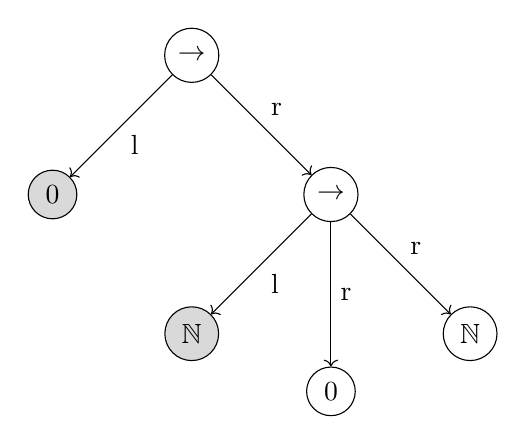
\begin{tikzpicture}[node distance={25mm}, main/.style = {draw, circle}]
    \node[main] (1) {$\to$};
    \node[main, fill=gray!30] (2) [below left of=1] {$\Singleton{0}$};
    \node[main] (3) [below right of=1] {$\to$};
    \node[main, fill=gray!30] (4) [below left of=3] {$\Nat$};
    \node[main] (5) [below right of=3] {$\Nat$};
    \node[main] (6) [below of=3] {$\Singleton{0}$};
    \draw[->] (1) edge["l"] (2);
    \draw[->] (1) edge["r"] (3);
    \draw[->] (3) edge["l"] (4);
    \draw[->] (3) edge["r"] (5);
    \draw[->] (3) edge["r"] (6);
  \end{tikzpicture}
  \caption{Type automaton for $\Singleton{0} \to (\Nat \to \Singleton{0} \join \Nat)$}
  \label{fig:example-type-automaton}
\end{figure}

\begin{itemize}
  \item We create a type automaton $G = (q_0, N, E, \delta)$
  \item We construct the intersection automaton as $G_\cap = \dots$
  \item We check whether $G_\cap$ accepts the empty language, i.e. represents the empty type $\bot$
\end{itemize}

\subsubsection{Constructing type automata}
\subsubsection{Minimizing type automata}


\subsection{Rest}
We should always check in an instance declaration whether this constraint globally holds. \\
To guarantee modularity we also have to check this for module imports, but since even the import of functions using different instances for the same type can lead to incoherences, we have to rule out any declaration of orphan instances.
\cite{Kilpatrick2019-cy}.
\cleardoublepage

%%
%%%%%%%%%%%%%%%%%%%%%%%%%%%%%%%%%%%%%%%%%%%%%%%%%%%%%%%%%%%%%%%%%%%%
% Diskussion und Ausblick
%%%%%%%%%%%%%%%%%%%%%%%%%%%%%%%%%%%%%%%%%%%%%%%%%%%%%%%%%%%%%%%%%%%%

\chapter{Summary}
  \label{ch:summary}


\clearpage

\cleardoublepage

%%
% %%%%%%%%%%%%%%%%%%%%%%%%%%%%%%%%%%%%%%%%%%%%%%%%%%%%%%%%%%%%%%%%%%%%
% Diskussion und Ausblick
%%%%%%%%%%%%%%%%%%%%%%%%%%%%%%%%%%%%%%%%%%%%%%%%%%%%%%%%%%%%%%%%%%%%

\chapter{Discussion and Outlook}
\label{ch:discussion}

\section{Future Work}

\subsection{Multi Parameter Type Classes}

The concrete implementation may impose further restrictions on instance resolution.

Our language differentiattes covariant and contravariant type classes.
This distinction is made for the type variable declared in the class declaration.

In a covariant type class, type variables may only occur on covariant positions in the class methods signatures.
A simple example for a covariant type class is the \mintinline{Haskell}{Show} class:

\begin{minted}{Haskell}
  class Show +a where
    show :: a -> String
\end{minted}

Dually in a contravariant type class, type variables may only occur on contravariant positions in the class methods signatures.
A simple example for a contravariant type class is the \mintinline{Haskell}{Read} class:

\begin{minted}{Haskell}
  class Read -a where
    read :: Read -> a
\end{minted}

This distinction imposes a problem when we want to implement type classes in which the type variable may occur both in a covariant and contravariant position.

\begin{minted}{Haskell}
  class Semigroup a where
    mappend :: a -> a -> a
\end{minted}

One way to solve this problem is by distinguishing covariant and contravariant type variables.
We can do so by introducing multi parameter type classes:

\begin{minted}{Haskell}
  class Semigroup +a -b where
    mappend :: a -> a -> b
\end{minted}

Instead of defining an instance for \mintinline{Haskell}{Semigroup Nat}, we would then have to define an instance for \mintinline{Haskell}{Semigroup Nat Nat}.
The latter seems to be less intuitive because semigroups are not a relation between types but a property for just one type (the operator has to map two elements from one set into the same set).
Since such cases may occur in many other classes (e.g. Num, Monad) it may be helpful to define syntactic sugar for type classes with mixed variance.
Then, the less intuitive implementation as multi parameter type classes could be hidden on the surface syntax.

Discuss instance chains:
We can relax this constraint by defining an explicit order in which instances should be picked/resolved.
\cite{morris2010instance}

\cleardoublepage


%%%%%%%%%%%%%%%%%%%%%%%%%%%%%%%%%%%%%%%%%%%%%%%%%%%%%%%%%%%%%%%%%%%%%%%%%%%%%
%%% Appendix
%%%%%%%%%%%%%%%%%%%%%%%%%%%%%%%%%%%%%%%%%%%%%%%%%%%%%%%%%%%%%%%%%%%%%%%%%%%%%
\appendix



\cleardoublepage

%%%%%%%%%%%%%%%%%%%%%%%%%%%%%%%%%%%%%%%%%%%%%%%%%%%%%%%%%%%%%%%%%%%%%%%%%%%%%
%%% Bibliographie
%%%%%%%%%%%%%%%%%%%%%%%%%%%%%%%%%%%%%%%%%%%%%%%%%%%%%%%%%%%%%%%%%%%%%%%%%%%%%

\addcontentsline{toc}{chapter}{Bibliography}

\bibliographystyle{alpha}
\bibliography{literature}

\cleardoublepage
%%%%%%%%%%%%%%%%%%%%%%%%%%%%%%%%%%%%%%%%%%%%%%%%%%%%%%%%%%%%%%%%%%%%%%%%%%%%%
%%% Erklaerung
%%%%%%%%%%%%%%%%%%%%%%%%%%%%%%%%%%%%%%%%%%%%%%%%%%%%%%%%%%%%%%%%%%%%%%%%%%%%%
\thispagestyle{empty}
\section*{Selbst\"andigkeitserkl\"arung}

Hiermit versichere ich, dass ich die vorliegende Masterarbeit 
selbst\"andig und nur mit den angegebenen Hilfsmitteln angefertigt habe und dass alle Stellen, die dem Wortlaut oder dem 
Sinne nach anderen Werken entnommen sind, durch Angaben von Quellen als 
Entlehnung kenntlich gemacht worden sind. 
Diese Masterarbeit wurde in gleicher oder \"ahnlicher Form in keinem anderen 
Studiengang als Pr\"ufungsleistung vorgelegt. 

\vskip 3cm

Ort, Datum	\hfill Unterschrift \hfill 
%%%%%%%%%%%%%%%%%%%%%%%%%%%%%%%%%%%%%%%%%%%%%%%%%%%%%%%%%%%%%%%%%%%%%%%%%%%%%
%%% Ende
%%%%%%%%%%%%%%%%%%%%%%%%%%%%%%%%%%%%%%%%%%%%%%%%%%%%%%%%%%%%%%%%%%%%%%%%%%%%%

\end{document}

